\chapter{Discussion}
Throughout this thesis, there have been numerous assumptions and uncertainties, some of which have been commented on and some left untouched. This chapter aims to address and comment on these in greater detail and discuss how such factors could influence the results. Although it is perplexing to comprehend the propagation of uncertainties, we wish to discuss the general validity and debate how further research could improve the results. 

%%%%%%%%%%%%%%%%%%%%%%%%%%%%%%%%%%%%%%%%%%%%%%
\section{General validity}
In chapter \ref{chap:analysis}, it was determined that a power increase of nearly eight percent was possible at both distances for certain combinations of control parameters. Although this is a relatively significant improvement, it still seems intuitively plausible to achieve. It is nice to see results that do not contradict our intuition, but still a vague argumentation for the validity from a scientific standpoint. To check whether the network output and optimization make any physical sense, we will look at a direct time series at one of the better configurations and see how the turbines behave. The closest simulation we have to the optimal point for the distance of $6R$ is case 9, where we have the following control parameters. 

\begin{equation*}
    \psi_1=-25^\circ, \quad \Omega_1=0.84 rad/s, \quad \theta_1 = 1.3^\circ, \quad \psi_2 = 4^\circ
\end{equation*}

Taking an arbitrary time series and plotting the power production of both turbines with the power for normal operation yields the graph displayed in figure \ref{fig:powertimeseries}

\begin{figure}[H]
    \centering
    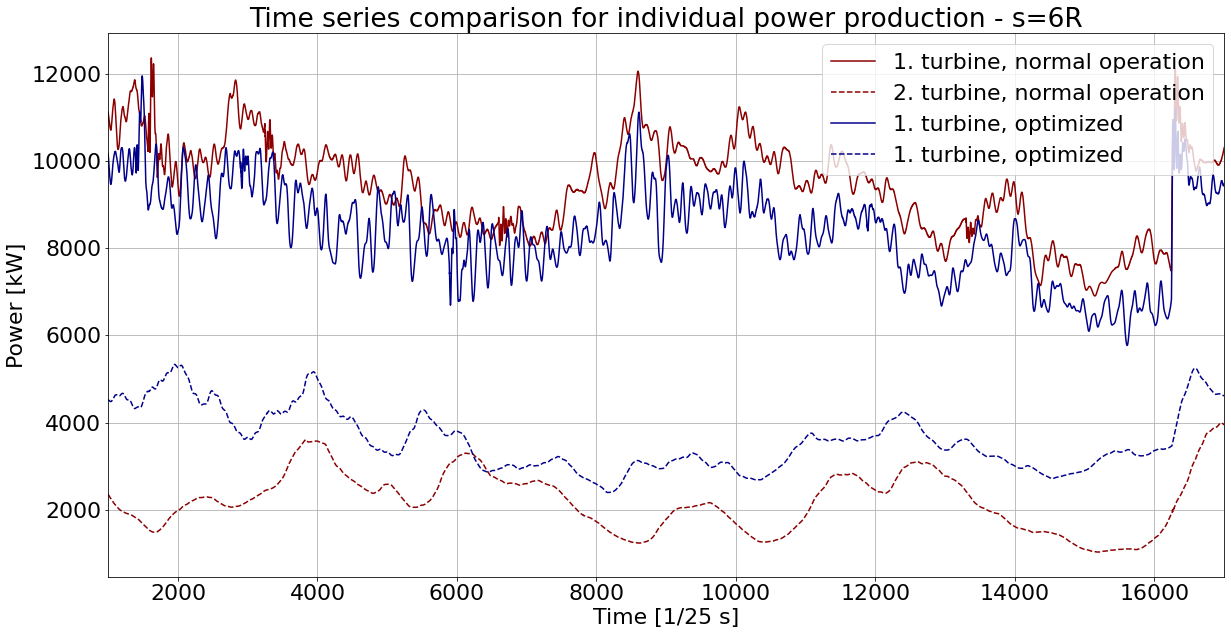
\includegraphics[scale=0.26]{Illustrations/Timeseries_y1=-25_o1=85_p1=130_s6R_y2=4.png}
    \caption{Power time series for $\psi_1=-25^\circ, \; \Omega_1=0.84 rad/s, \; \theta_1 = 1.3^\circ, \; \psi_2 = 4^\circ$}
    \label{fig:powertimeseries}
\end{figure}

As seen, the power reacts exactly how we expect. For the first turbine, the power decreases as we yaw the turbine, but in return, the second turbine dramatically improves its performance. Notably, the second turbine is significantly worse than the first, and the wake effects are still highly present. It is difficult to interpret whether the improvement makes up for the exacerbation of the first turbine, so it makes sense to look at the combined power instead. This plot for the same turbines is seen in figure \ref{fig:powertimeseries_total}.


\begin{figure}[H]
    \centering
    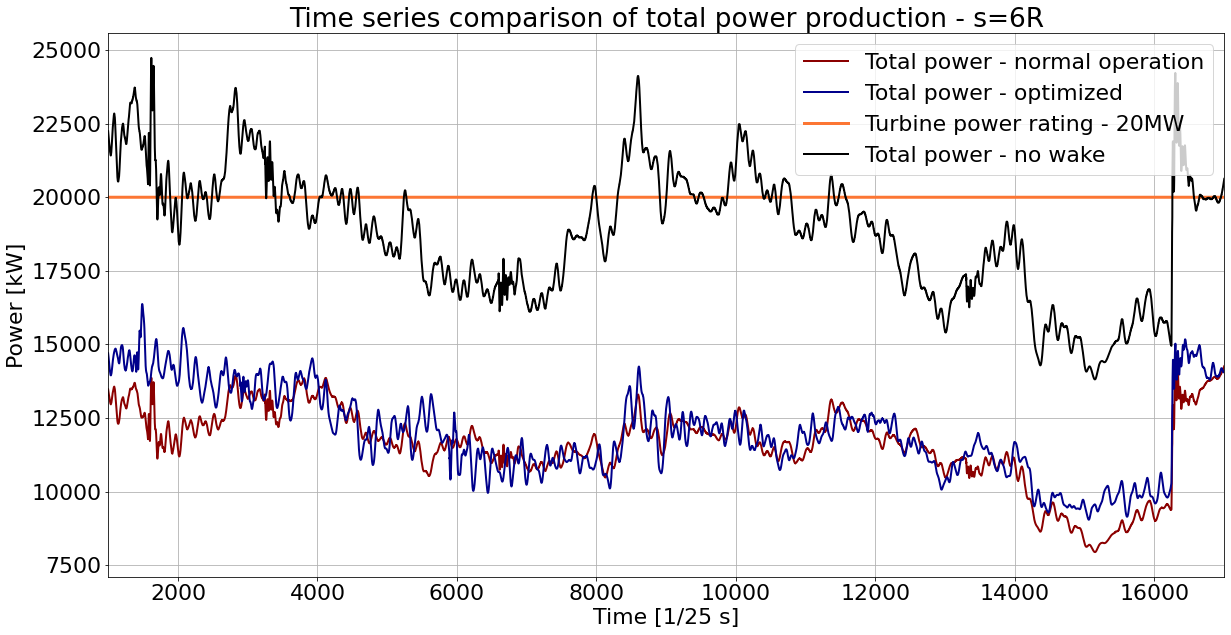
\includegraphics[scale=0.26]{Illustrations/Timeseries_y1=-25_o1=85_p1=130_s6R_y2=4_total.png}
    \caption{Combined power time series for $\psi_1=-25^\circ$,  $\Omega_1=0.84 rad/s$, $\theta_1 = 1.3^\circ,$ $\psi_2 = 4^\circ$}
    \label{fig:powertimeseries_total}
\end{figure}

At first glance, it seems that the combined power is almost interchangeable, but this makes sense considering that we expect a maximum of eight percent difference between them. Additionally, we see that the optimized case is performing slightly better at certain points, especially at the start and end of the period. As seen in the figure, we also plotted theoretical power without wake losses, which fluctuates around the rated value of $20MW$. What is important to realize is that the loss is much greater than the improvement, and it, therefore, sounds realistic that one could gain a small increase by steering the wake. Ultimately we do not see any indication that the calculations should be incorrect, and we should instead discuss how accurate we expect them to be. 

%%%%%%%%%%%%%%%%%%%%%%%%%%%%%%%%%%%%%%%%%%%%%%%%%%%%%%%%%%%
\section{Comparison with previous studies}

A recent paper by Debusscher \cite{charles} did a similar analysis for a much smaller turbine \cite{smallturbine}. His analysis determined that the maximum power gain available was just under three percent, at a distance of $6R$. In chapter \ref{chap:analysis}, we saw results of approximately eight percent, which is a substantial deviation relative to his results. What is notable in that comparison is that the optimal yawing angle of the first turbine, for maximum power, in his paper was approximately $23$ degrees. This suggests that our turbine \cite{turbineref} is less sensitive to yawing, which would explain both the higher power gain and the high value for the optimal angle. For the loads, it seems that Debusscher \cite{charles} generally determined a higher increase, for the optimised case, of about $10\%$ and $40\%$ on the first and second turbine, respectively. In this thesis, we considered loads as a collective quantity, which partly explains the difference. The remaining deviation is most likely due to the different turbines, although it might make sense to investigate this further.

%%%%%%%%%%%%%%%%%%%%%%%%%%%%%%%%%%%%%%%%%%%%%%%%%%%%%%%%%%%
\section{Uncertainties}

Starting by recognizing the most significant uncertainties and creating an overview of how they affect each other, we can comment on them chronologically.

\subsection{Use of mechanical power}

From the way the data is simulated through Flex5, we need to recognize a fundamental difference between the first and second turbine. For this analysis, the Flex5 calculations were based on the flow data for both turbines, but it is also possible for the first turbine to be directly coupled to the actuator lines. Wanting to alter control parameters on one turbine creates a problem since we are forced to turn off the controller, meaning that the electrical power cannot be directly extracted. Instead, we must calculate the mechanical power from the torque and rotational speed, as seen in equation \ref{powerequation}. The problem with this approach is that the turbine cannot convert all the mechanical power to electrical energy. Although it would be simple to correct for this imperfection, if we assumed the relative loss constant, there was not enough time in this project to repeat the simulations. Therefore, the actual power production will be slightly lower than portrayed whenever the first turbine is involved. However, since this is the case throughout the thesis, it should not matter significantly since it will more or less cancel out during the comparisons. It would be a definite implementation for future work, but for now, we assume that it does not have any significant impact on the results.

\subsection{Weibull fitting}
In section \ref{sec:Aeroelastic}, it was decided to use a Weibull CDF fit to represent the data. This was necessary to reduce computational time, as the available resources could not handle the available data. In total, this assumption reduced the simulated data from approximately 1.640.000.000 to 4.500 data points by representing each time series as an average and each collection of averages as a cumulative distribution function. One thing to note is the original data fluctuations have not been considered. From figure \ref{fig:flap_load_example}, however, these seem relatively consistent, so we assume this to be a reasonable course of action for a long time series. It should also be commented that power has a $R^2$-value around 0.9 and still contains an uncertainty, which was completely disregarded for further analysis. As previously mentioned, this suggests that a Weibull is a good, but not perfect, fit. For future work, it might make sense to investigate if there are other more accurate ways to fit this distribution or find computers powerful enough to brute force the calculations. 

\subsection{Median/Mean}
Going from the Weibull representation to a more practical value for the turbine outputs, we could utilize two primary methodologies: the median and mean, respectively. For a Weibull distribution, the mean is generally larger, which is amplified the more separated the data gets. For the case of wind turbines, it seems reasonable to use the median since it represents the most common occurrence, but it would be interesting to see how using the mean would alter the results and if it would have any impact on the optimal configurations. 


\subsection{Network accuracy}

In chapter \ref{Surrogates} a relatively simple network was applied. Though the accuracy of test data seen in figure \ref{fig:boxplotacc} is relatively high, we still have some outliers of up to two percent. This is not insignificant when combined with the uncertainty from the distribution. An obvious way to enhance this performance would be to simulate additional data or model a more complex network. 


\subsection{Distances}

In chapter \ref{chap:analysis}, we looked at two distances of $6R$ and $14R$, representing a short and normal distance, respectively. The choice of distances was primarily based on the results of a previous study \cite{charles}, which turned out not to be as similar as expected. It would therefore be interesting to do a similar analysis and see how this turbine changes behaviour over a broader range of distances. 



\subsection{Prediction steps}

When plotting the contour plots in chapter \ref{chap:analysis}, we saw some interesting behaviour of the load plots for the optimized parameters. As previously mentioned, this could be smoothed out by refining the optimization but has not been done as a limitation of the available resources. Currently, each of the six contours is based on 1.891 points of yawing combinations, each evaluated on 56 combinations of $\Omega_1$ and $\theta_1$. This requires approximately 106.000 network predictions per graph, which equals multiple hours of computation on a high-performance computer. The number of predictions would quadruple should we wish to double the number of steps for both $\Omega_1$ and $\theta_1$, which is not practical to compute. For future work, it might make sense to compute a refined version on a designated server and create a smoother plot. It might also make sense to investigate which parameter changes across these lines and relate this to a physical understanding. 

\subsection{Simulation data}
\label{sec:Simulation_discussion}

A notable trend from chapter \ref{chap:analysis} is that the maximum power gain was consistently at the maximum yawing angle of the first turbine, at the distance of $6R$. This is not something we wish to see since there might be a more optimal point that we have not investigated. Unfortunately, neural networks generally perform very poorly when predicting outside the range of the training data. Therefore, we cannot expect accurate results if we explore a broader range since the simulation data is limited from -30 to 0 degrees. For future work, it will be essential to perform more CFD simulations, which will enable us to investigate this, as well as increase the network accuracy in general. It would also make sense to apply the knowledge found in this thesis to better determine the configurations for new simulations. For example, it seems unnecessary to simulate more cases with different rotational speeds when we expect this to be constant. However, yawing and pitching found values at the end of the range and should therefore be expanded. 




